\chapter{自然语言处理}

\section*{Introduction}
	本章节主要介绍一些文本方面相关的知识。
	
\section{如何表示词}
	\subsection*{Introduction}
	本节主要介绍如何使用词向量的形式去表达一个模型,本章节大部分内容来自知乎专栏以及cs224d课程。
	
	准备重写这一部分的内容,整个符号体系沿用cs224n课程的符号体系,说明如下:
	
	\begin{itemize}
		\item V表示中心词矩阵,其中的每一列$v_i$表示第i个中心词的词向量。
		\item U表示输出词矩阵,其中的每一列$u_i$表示第i个上下文词的词向量,为V的转置。
		\item 我们使用$w_t$,来表示第t个词,这里不却分中心词和上下问的词。
		\item 用T来表示词表,|T|来表示此表中词的个数
	\end{itemize}
	
	\subsection{one-hot}
	首先,可以将每个词表示成one-hot vector,就是只有在对应位置的向量的值为1,其余位置为0,如下图所示:
	

	\begin{figure}[htbp]
	\centering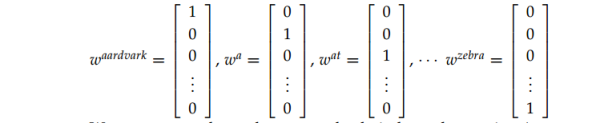
\includegraphics[width=6in]{img/6-1.png}
	\caption{one-hot}\label{fig:6-1}
	\end{figure}
	
	但是这种表示方法有几种缺点,一种是如果词表太长的话,我们可能没有那么多的内存去存储这么多的词向量,另外一种是,每个word之间都是独立的,我们没有办法从中找到他们之间的关系。
	
	\begin{equation}
	(w^{hotel})^{T}(w^{motel}) = (w^{hotel})^{T}(w^{cat})=0
	\end{equation}
	
	虽然两个向量之间的点乘可以表示word之间的关系,但是由于在one-hot中,任意两个向量都是正交的,因此他们之间的点乘结果都是0,所以不能通过这种方式来表达向量之间的相似程度。因此我们需要通过某种方式,将这个高维空间压缩到一个低维的空间中去。	
	
	比如,我们可以通过一个词周围的词来表达这个词的信息。比如如下的例子。可以用banking周围的词来代表banking这个词,这样在大规模的预料中,这样的统计就变得比较重要了。
	
	\begin{figure}[htbp]
	\centering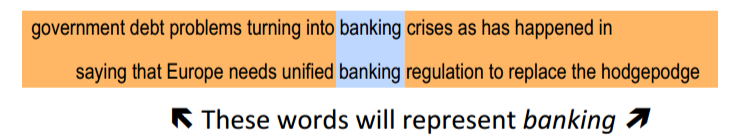
\includegraphics[width=6in]{img/6-2.png}
	\caption{词的表示形式}\label{fig:6-2}
	\end{figure}
	
	这样,我们就可以将之前的one-hot形式的稀疏矩阵变成一个稠密的矩阵了,但是这里的一个词的词向量是从计算机的角度来理解的,没有什么感知上的意义。这样,我们的问题就比较明确了,即找到一个model来刻画一个词和它的上下文之间的概率(即将one-hot变成稠密的矩阵),概率越大说明学习的越好。如果取负值,那么这就是我们的loss function 了。
	
	
	\subsection{skip-gram}
	
	skip-gram是word2vec的其中一种方法,主要的目的是找到一个词和它的上下文之间的关联。word2vec主要有两种模型,两种训练的方法。
	
	skip-gram是一种根据当前的word预测contex的算法。
	
	我们使用如下所示的图来表示skip-gram,加入中心词banking的位置为t,那么我们分别根据第t个词来预测第t-m,...t-1,t+1,...,t+m个词的概率。其中除了第t个词的其他的词叫做output context words。每次计算的时候,取一个词作为中心词
	
	\begin{figure}[htbp]
	\centering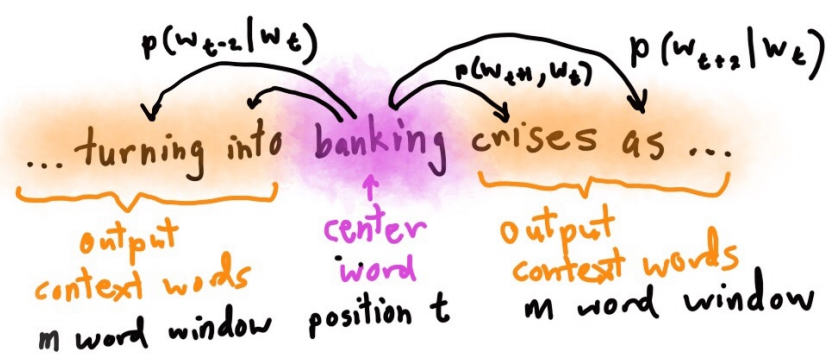
\includegraphics[width=6in]{img/6-3.png}
	\caption{skip-gram}\label{fig:6-3}
	\end{figure}
	
	这样我们就可以获得skip-gram的计算公式了,即分别计算已知第t个词,预测前后m个词的概率,然后最大化概率的成绩即可,对于第二个连乘来说计算的是这一个中心词的所有上下文词的概率,第一个连乘表示的是每次取一个词作为中心词,遍历所有的词。加入负号之后我们即可以直接作为loss function 来使用了。公式如下:
	
	\begin{equation}
		L(\theta) = \prod_{t=1}^{T} \prod_{-m \leq j \leq m} p(w_{t+j}|w_t;\theta)
	\end{equation}
	
	\begin{equation}
		J(\theta) = -\frac{1}{T} \sum_{t=1}^{T} \sum_{-m \leq j \leq m} \log p(w_{t+j}|w_t)
	\end{equation}
	
	通常我们是使用交叉熵来作为损失函数,但是这里的向量使用的是one-hot的形式,计算结果时只有trueclass的位置有值,这样显得不太妥当。
	
	这样我们已经获得了损失函数,下面我们需要做的就仅仅是求出这样一个概率就可以了。概率可以使用如下的公式来求解。同样首先我们需要定义一些表达式:c表示中心词的下标;$v_c$表示第c个中心词的词向量,$u_o$表示第o个outside词的词向量。这样我们就可以表示已知第c个词求第o个词的概率:(这里我们用的是点积,即每个向量对应位置的元素相乘。点乘的意义是两个向量越是接近,点乘的结果越大)
	
	这个公式其实就是算出中心词和每一个上下文词的相似度,相似度就是两个词的词向量的点积,$u_wv_c$,其中$u_o$就是第w个上下文词,$v_c$代表当前的中心词,这里的$p(o|c)$表达的是第o个上下文词与第v个中心词中间的关系,但是我们最后需要求出所有的上下文词与中心词之间的关系,因此根据下文中的推倒过程我们可以观察到,我们需要对o进行遍历(从1到|T|),来获得我们想要的结果。
	
	\begin{equation}
	p(o|c) = \frac{exp(u_0^T v_c)}{\sum_{w=1}^v exp(u_w^T v_c)}
	\end{equation}
	
	\begin{figure}[!htbp]
	\centering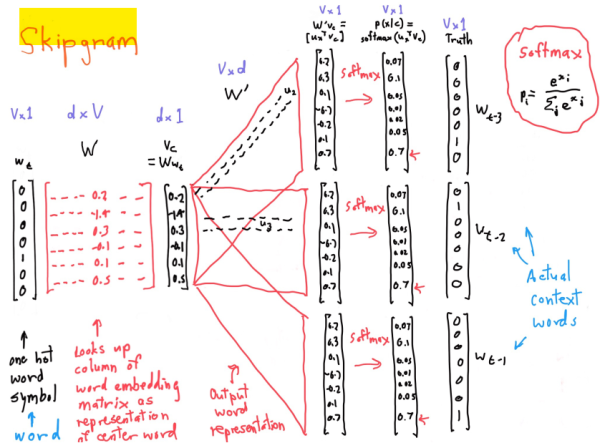
\includegraphics[width=5.5in]{img/6-4.png}
	\caption{skip-gram}\label{fig:6-4}
	\end{figure}
	
	
	需要注意的是,我们通常初始化的时候U和V(即输出词矩阵和中心词矩阵)都是随机初始化的,我们是在梯度下降的时候对这两个矩阵进行更新,最后网络的输出结果就是这两个矩阵,我们最终也仅仅是需要知道这两个矩阵即可,其他的像是损失函数以及网络的输出结果都是我们不关心的,之所以需要有这两个东西,就是为了获得输出词矩阵和中心矩阵。下面的几页ppt讲述了梯度下降的过程中是如何求解$v_c$的,即第c个中心词的词向量。输出词矩阵也是按照如下的方式方向传播,只不过符号不同而已。
	
	下面,我们介绍如何通过反向传播算法求解skip-gram。
	
%	\begin{equation}
%		J(\theta) = -\frac{1}{T} \sum_{t=1}^{T} \sum_{-m \leq j \leq m} \log p(w_{t+j}|w_t)
%	\end{equation}
%	
%	\begin{equation}
%	p(o|c) = \frac{exp(u_0^T v_c)}{\sum_{w=1}^v exp(u_w^T v_c)}
%	\end{equation}
%	
%	如果我们要对$J(\theta)$求导的话,其实相当于对$\log(p(o|c))$来求导,公式如下:
%	\begin{align*}
%		\frac{\partial J}{\partial v_c}
%		& = \frac{\partial log(\frac{exp(u_o^Tv_c)}{\sum_{w=1}^{|T| exp(u_wv_c)}})}{\partial v_c}
%		& = \frac{\partial \log (exp(u_o^Tv_c))}{\partial v_c} - \frac{\partial \log \sum_{w=1}^{|T|}(exp(u_o^Tv_c))}{\partial v_c}
%	\end{align*}


	\begin{figure}[!htbp]
	\centering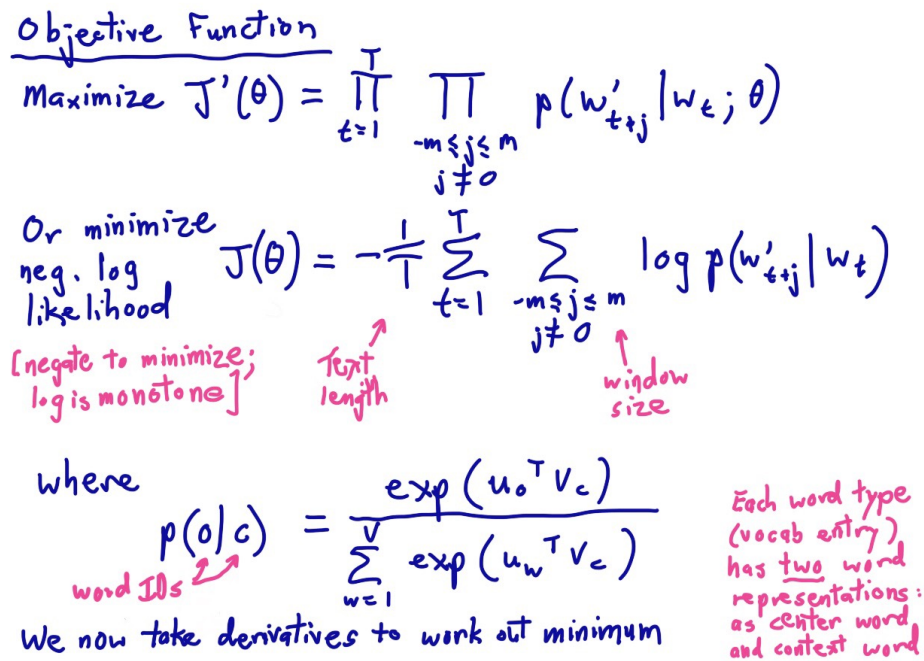
\includegraphics[width=6.5in]{img/6-5.png}
	\caption{目标}\label{fig:6-5}
	\end{figure}	
	
	\begin{figure}[!htbp]
	\centering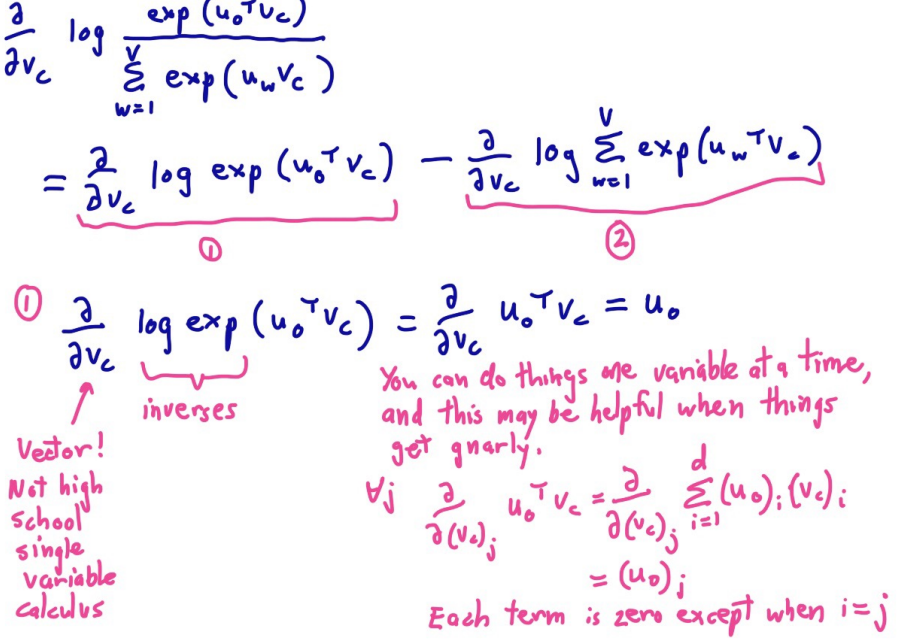
\includegraphics[width=6.5in]{img/6-6.png}
	\caption{反向传播}\label{fig:6-6}
	\end{figure}
	\begin{figure}[!htbp]
	\centering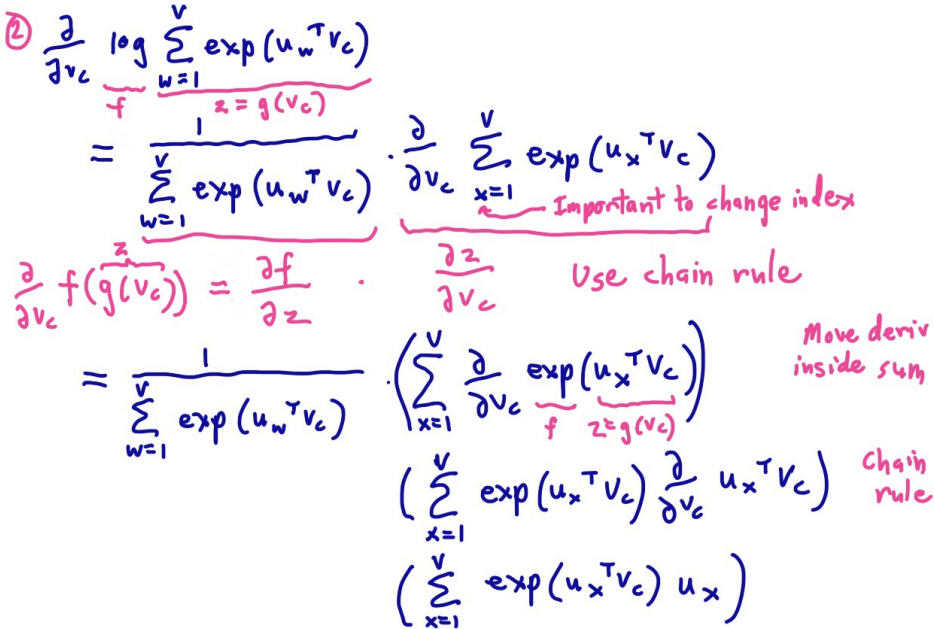
\includegraphics[width=6.5in]{img/6-7.png}
	\caption{反向传播}\label{fig:6-7}
	\end{figure}
	
	\begin{figure}[!htbp]
	\centering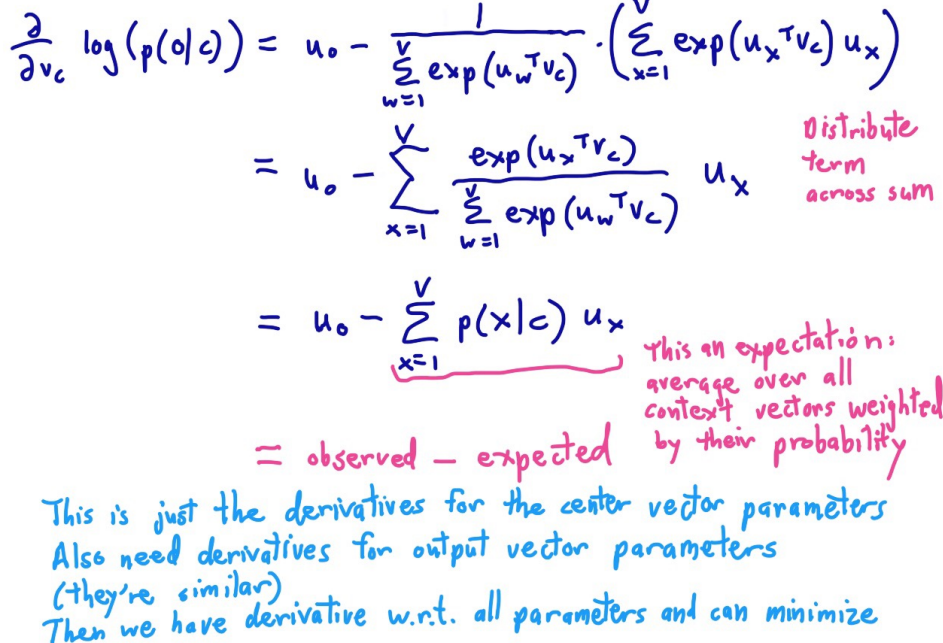
\includegraphics[width=6.5in]{img/6-8.png}
	\caption{反向传播}\label{fig:6-8}
	\end{figure}
	
	其中m表示我们的窗口的大小
	需要注意的是:在每一个窗口,我们更新这个窗口所遇到的所有的参数。如假设我们的窗口为1,要处理的文本为 we like leaing a lot , 第一个窗口我们需要计算internal vector $v_{like}$ 和external vector          $u_{we},u_{learing}$,第二个窗口的计算也是这样的。
	
	
	
	\subsection{Negatibe Sample}
	
	假如我们有这样一句话: I love deep learing and NLP
	
	在使用skip-gram的时候,假设第一个中心词为love,窗口大小m=1,那么我们首先需要从center word matrix V中取出一列$v_{love}$,然后从output word matrix U中取出一列$u_I$来计算概率$p(I|love) = \frac{exp(u_I^Tv_{love})}{\sum_{w=1}^V u_w^T v_{love}}$,这个公式中的V代表词表中的所有的词,然后从center word matrix V中取出一列$v_{love}$,然后从output word matrix U中取出一列$u_{deep}$来计算概率$p(deep|love) = \frac{exp(u_I^Tv_{love})}{\sum_{w=1}^V u_w^T v_{love}}$,这样当love作为中心词的时候我们需要计算的概率就已经计算完了。我们可以通过这种方式继续计算当deep为中心词,以及后面的词为中心词的所有情况所需要的概率。
	
	那么这样做有什么缺点呢?在计算概率的时候,分母中我们需要计算每一个词表中的词与当前中心词的相似度,当词表变得很大的时候,这样的计算量明显是很吃内存的,并且大量的词与中心词是没有任何关系的,因此我们需要简化这样的操作。
	
	
	在cs224n中只介绍了这么多,所以暂时只写这么多.
	
	在上一节的内容中我们推导出了word2vec的损失函数是:
	
	\begin{equation}
	J(\theta) = -\frac{1}{T} \sum_{t=1}^{T} J_t(\theta) 
	\end{equation}
	
	在这里我们用$\theta$表示损失函数中所有的参数,这里是U和V,其中$J_t(\theta) $为:
	
	\begin{equation}
	J_t(\theta) = \log \sigma(u_o^T v_c) + \sum_{i=1}^{k}E_{j=P(w)}[\log \sigma(u_j^T v_c)]
	\end{equation}
	
	k表示我们使用的要进行负采样的个数。这里我们是使用的$J_t(\theta)$来代替了之前所使用的log概率。之所以这样做是因为我们要最大化真正的outside word词在$v_c$附近出现的概率,而最小化我们随机选择的词在$v_c$附近出现的概率。
	
	还有一个需要注意的是,在那篇原始论文中也出现过一次,就是这里的$P(w)=U(w)^(3/4)/Z$,暂时不清楚是什么意思。$p(w)$表示的是noise distribution,这里的$U(w)$表示的是unigram distribution。待补充
	

	
	\subsection{CBOW}
	CBOW根据surrounding context 来预测center word,对于每一个词,需要学习两个vector,v(input vector):when the word is in the context;u(output):when the word is in the center.
	
	以上其实就基本是是word2vec的所有内容了。word2vec最终可以获得很多相邻的词,如果我们可以将结果可视化出来的话,对于一个词来说,我们可以获得经常与这个词一起出现的词,比如对于google通常会和yahoo一起出现一样。
	
	word2vec的本质就是预测每一个词的周围的词,那么这也有很大的缺点,比如我们每次只计算一个词周围的词,造成了时间上的浪费。
	
	那么有没有其他的解决方案呢?比如一次预测多个词,当然有!!!
	
	
	\subsection{基于SVD的方法}
	
	\subsubsection{window based co-occurrence matrix}
	
	对于如下三句话来说,我们的窗口大小是1(通常来说是5-10),是对称的(即词出现在中心词的左边和右边都是没有关系的),但是在这一类算法中,并不是总是对称的
	
	I like deep learing
	
	I like NLP
	
	I enjoy flying
	
	
	对于这种算法,我们只要统计出如下的表格就可以了
	
	\begin{figure}[!htbp]
	\centering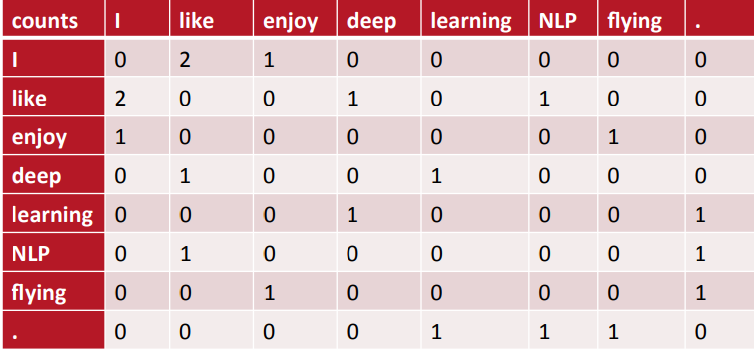
\includegraphics[width=6.5in]{img/6-9.png}
	\caption{统计表格}\label{fig:6-9}
	\end{figure}
	
	但是这样做也有着明显的缺点,比如我们的存储会随着此表的大小而逐渐的变大,模型不够鲁棒等。因此我们很需要对数据进行降维。
	
	\subsubsection{low dimensional vector}
	
	在这里我们将所有的词表中出现的词存储到一个固定的低维的向量中去,通常为25-1000维,降维方法使用PCA。
	
	改进
	
	\begin{itemize}
		\item 有一些经常出现的词,比如the,he等?这种情况我们可以让最大的count=100,再大就不再增加了,或者直接忽略掉这些词	
		\item  使用皮尔逊系数来代替counts,然后把负样本的值标记为0
		\item 根据与中央词的距离衰减词频权重
	\end{itemize}
	
	使用SVD表示词向量的方法虽然比较简单,但是效果也还不错。这样的方法以及效果,在这篇论文中有详细的介绍An	Improved Model of SemanRc Similarity Based on Lexical	Co-Occurrence Rohde	et al. 2005
	
	但是使用SVD表示词向量有着各种各样的问题,比如计算复杂度比较高,不方便处理新词或者新的文档,与其他的DL模型的训练套路不同。
	
	因此提出了一种结合了word2vec和SVD两种方法的新方法提出来了,GloVe方法。
	
	
	\subsection{GloVe}
	
	Glove的目标函数是:
	
	\begin{equation}
	J(\theta) = \frac{1}{2} \sum_{i,j=1}^{W} f(P_{ij})(u_i^Tv_j-\log P_{ij})^2
	\end{equation}
	
	其中,$P_{ij}$表示第i和第j个词共同出现的频率,f是一个max函数,图像如下图所示
	
	
	\begin{figure}[!htbp]
	\centering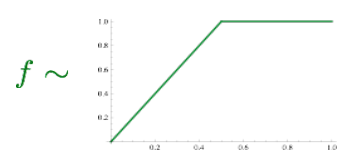
\includegraphics[width=4in]{img/6-10.png}
	\caption{f函数}\label{fig:6-10}
	\end{figure}
	
	P是在一开始就计算好的一个矩阵,$f(P_{ij})$是控制该对词的权重,贡献次数越大,权重也越大,但是当大于一个阈值后,权重为1,不再变化。后面的square loss ,目的是希望频次过高时,两者的相似度也大,这样使得整体loss变小。
	
	Glove的优点是训练快,可以扩展到大规模语料,也适用于小的语料和向量
	
	另外在损失函数中,我们发现u和v都捕捉到了共现信息,那么我们可以将他们直接加起来作为我们的信息$X_{final} = U + V$,相对于word2vec来说,只关注一个窗口内相近的词出现的频率,但是Glove更关注全局上两个词出现的频率。
	
	\subsection{评价方法}
	
	Intrinsic:专门设计单独的试验,由人工标注词语或句子相似度,与模型结果对比。好处是是计算速度快,但不知道对实际应用有无帮助。有人花了几年时间提高了在某个数据集上的分数,当将其词向量用于真实任务时并没有多少提高效果,想想真悲哀。
	
	通过a对于b来讲,相当于c对于哪个词?主要通过如下的公式来获得
	
	\begin{figure}[!htbp]
	\centering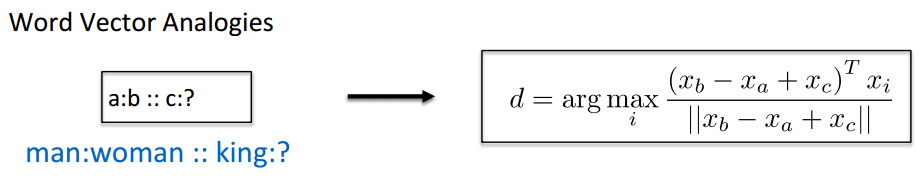
\includegraphics[width=6in]{img/6-11.png}
	\caption{intrinsic word vector evalution}\label{fig:6-11}
	\end{figure}
	
	比如man:woman::king:? 这种结果可视化出来后,往往都是平行的向量

	Extrinsic:通过对外部实际应用的效果提升来体现。耗时较长,不能排除是否是新的词向量与旧系统的某种契合度产生。需要至少两个subsystems同时证明。这类评测中,往往会用pre-train的向量在外部任务的语料上retrain。
	
	\subsubsection{调参}
	如果考虑到成本的话,大约300维,窗口为8的对称窗口的效果是最好的
	
	\begin{figure}[!htbp]
	\centering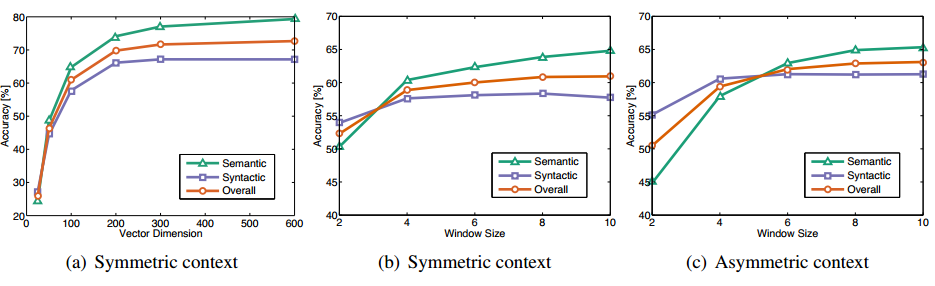
\includegraphics[width=6in]{img/6-12.png}
	\caption{调参}\label{fig:6-12}
	\end{figure}
	
	
\section{文本分类}
	\subsection*{Introduction}
	本章内容主要介绍一些基本概念
	
	\subsection{Softmax}
	
	
	
	
	
	
	
	
	
	
	
	
	
	
	
	
	
	
	
	
	
	
	
	
	
	
	
	
	
	
	
	
	
	    	
	
	